% This is "sig-alternate.tex" V2.0 May 2012
% This file should be compiled with V2.5 of "sig-alternate.cls" May 2012
%
% This example file demonstrates the use of the 'sig-alternate.cls'
% V2.5 LaTeX2e document class file. It is for those submitting
% articles to ACM Conference Proceedings WHO DO NOT WISH TO
% STRICTLY ADHERE TO THE SIGS (PUBS-BOARD-ENDORSED) STYLE.
% The 'sig-alternate.cls' file will produce a similar-looking,
% albeit, 'tighter' paper resulting in, invariably, fewer pages.
%
% ----------------------------------------------------------------------------------------------------------------
% This .tex file (and associated .cls V2.5) produces:
%       1) The Permission Statement
%       2) The Conference (location) Info information
%       3) The Copyright Line with ACM data
%       4) NO page numbers
%
% as against the acm_proc_article-sp.cls file which
% DOES NOT produce 1) thru' 3) above.
%
% Using 'sig-alternate.cls' you have control, however, from within
% the source .tex file, over both the CopyrightYear
% (defaulted to 200X) and the ACM Copyright Data
% (defaulted to X-XXXXX-XX-X/XX/XX).
% e.g.
% \CopyrightYear{2007} will cause 2007 to appear in the copyright line.
% \crdata{0-12345-67-8/90/12} will cause 0-12345-67-8/90/12 to appear in the copyright line.
%
% ---------------------------------------------------------------------------------------------------------------
% This .tex source is an example which *does* use
% the .bib file (from which the .bbl file % is produced).
% REMEMBER HOWEVER: After having produced the .bbl file,
% and prior to final submission, you *NEED* to 'insert'
% your .bbl file into your source .tex file so as to provide
% ONE 'self-contained' source file.
%
% ================= IF YOU HAVE QUESTIONS =======================
% Questions regarding the SIGS styles, SIGS policies and
% procedures, Conferences etc. should be sent to
% Adrienne Griscti (griscti@acm.org)
%
% Technical questions _only_ to
% Gerald Murray (murray@hq.acm.org)
% ===============================================================
%
% For tracking purposes - this is V2.0 - May 2012

\documentclass{sig-alternate}

\usepackage{url}

\def\sharedaffiliation{
\end{tabular}
\begin{tabular}{c}}

\begin{document}
%
% --- Author Metadata here ---
%\conferenceinfo{WOODSTOCK}{'97 El Paso, Texas USA}
%\CopyrightYear{2007} % Allows default copyright year (20XX) to be over-ridden - IF NEED BE.
%\crdata{0-12345-67-8/90/01}  % Allows default copyright data (0-89791-88-6/97/05) to be over-ridden - IF NEED BE.
% --- End of Author Metadata ---

\title{Gang Scheduling Java Applications with Tessellation}

\numberofauthors{4}

\author{
Benjamin Le \and Jefferson Lai \and Wenxuan Cai \and John Kubiatowicz\titlenote{The Parallel Computing Laboratory, UC Berkeley, CA, USA}\\
      \sharedaffiliation
      \affaddr{\{benjaminhoanle, jefflai2, wenxuancai\}@berkeley.edu, kubitron@cs.berkeley.edu}\\
      \affaddr{Department of Electrical Engineering and Computer Science }\\
      \affaddr{University of California, Berkeley }\\
      \affaddr{Berkeley, CA 94720-1776}
}

\maketitle
\begin{abstract}
Java applications run within Java Virtual Machines (JVM). As an application runs, the JVM performs many parallel background tasks for general housekeeping reasons including garbage collection and code profiling for adaptive optimization. While this design works well to provide isolation when there is a single or small number of Java applications running on a single machine, in practice it is common to find a large number of Java applications running concurrently on a single machine. For example, a machine could be running multiple instances of HDFS, Hadoop, and Spark, simultaneously, with each instance having an associated JVM. As all of these JVMs must ultimately be multiplexed onto a single set of hardware, interference among the large set of parallel tasks arise. There is little published literature documenting the causes of this interference or how to deal with it. In this paper, we determine the specific sources of these interferences and show how running these applications on top of a Tessellation-integrated Xen hypervisor addresses these issues and reduces interference. We evaluate the performance of these “Tessellated” machines in comparison with machines running bare Linux when running a large number of JVMs.
\end{abstract}

% Same categories as Juan's DAC 2013 Tesselation paper
\category{D.4.1}{Operating Systems}{Process Management -- Scheduling}
\category{D.4.8}{Operating Systems}{Performance -- Measurements, Monitors}

\terms{Multicore, parallel, quality of service, resource containers}

\keywords{Adaptive resource management, performance isolation, quality of service}

\section{Introduction}

The Java Virtual Machine (JVM) abstraction provides a consistent, contained execution environment for Java applications and has played a significant role in Java's popularity and success in recent years. The JVM abstraction encapsulates many tasks and responsibilities that make development faster and easier. For example, by handling the translation of portable Java bytecode to machine code specific to the lower level kernel and system architecture, the JVM allows developers to write an application once and run it in a number of different environments. While there exist a number of JVM implementations, maintained both privately and publicly, in general, implementations adhere to a single JVM specification. We refer the reader to \cite{lindholm2014java} for a complete specification, but summarize the roles of two key, highly researched components of the JVM: the adaptive optimization component of the "just in time" (JIT) compiler and the garbage collector (GC) \cite{hotspot:whitepaper}.

The JIT compiler is responsible for compiling segments of bytecode into native machine instructions. Modern JIT compilers are extended with adaptive optimization techniques \cite{suganuma2001dynamic}, which attempt to optimize performance by dynamically compiling and caching these segments of code during run time. The result is a drastic performance improvement over simply interpreting the bytecode. Exactly how much compilation occurs before versus after a program begins executing and how much of a given program is interpreted varies across JVMs and significantly affects the performance characteristics of the program. While more advanced optimization results in higher performing code, it generally also requires more resources, including time, to perform, incurring higher overhead and impact on the program's performance.

Garbage collection is the process of cleaning up unused memory so that developers do not, and generally can not, manage memory themselves. While this makes development easier and can drastically reduce the number of memory related bugs, garbage collectors are very complex and, as with the adaptive optimization, consumes resources. Many techniques for garbage collection have been developed from simple reference counting, to parallelized stop-and-copy, to generational garbage collection \cite{lins1996garbage}. Each technique differs in how to locate "live" objects, when to run, whether and when execution needs to be halted, what memory needs to be touched, and how objects in memory should be moved.

Together, garbage collection and adaptive optimization require the JVM to perform many tasks background tasks in addition to program execution. While this design works well when there is a single or small number of Java applications on a machine, the same may not be true when there are a large number of Java applications running concurrently on a single machine. This type of situation can often be found within the machines in cloud computing clusters. Given the ubiquity of Java based software applications, as the popularity of distributed applications and the demand for cloud computing services increase, understanding the types of multi-tenancy issues that may arise becomes critical to progress. For example, a machine in the cloud could be asked to host multiple instances of Hadoop File System (HDFS) \cite{shvachko2010hadoop}, Hadoop MapReduce \cite{bialecki2005hadoop}, and Spark \cite{zaharia2010spark}, simultaneously, with each instance having a dedicated JVM. As all of these JVMs must ultimately be multiplexed onto a single set of hardware, significant interference may arise between the tasks of each JVM. For certain applications, for example those with strict timing requirements or quality of service (QoS) guarantees, this interference may lead to unacceptable performance.

%TODO Revist and update the last sentence (maybe paragraph) once we have results
In addition to investigating the significance of the issues named above, we consider a potential solution to interference that is made possible with the \textit{Tessellation} operating system architecture and the \textit{Adaptive Resource-Centric Computing (ARCC)} system design paradigm \cite{colmenares2010resource, colmenares2013tessellation, liu2009tessellation}. In ARCC, applications execute within stable, isolated resource containers called \textit{cells}. In addition to implementing cells, the ARCC-based Tessellation kernel uses \textit{two-level scheduling}, which decouples the allocation of resources to cells (the first level) from scheduling how these resources are used within cells (the second level). In this paper, we apply and evaluate gang scheduling \cite{feitelson1992gang} as a second level scheduling policy. In particular, we execute a single application and JVM in each cell and run multiple cells on a single, multi-core machine, gang scheduling each cell's resources together. By measuring the performance of these applications with and without gang scheduling, we show the effect of gang scheduling at mitigating interference for OpenJDK's HotSpot JVM.

The remainder of this paper is organized as follows. Section 2 provides background on the HotSpot JVM and the Tesselation architecture. Sections 3 and 4 describes our experimental setup and results with two Java different benchmark suites. In Section 5 we present a survey or related work. We discuss directions for future work in Section 6 and conclude in Section 7.

\section{Background}

This section provides an overview of the relevant features of OpenJDK's HotSpot JVM and of the primary features of the Tesselation manycore operating system.

\subsection{HotSpot}
There currently exist two primary implementations of the HotSpot JVM. One is owned and maintained privately by Oracle and the other is an open source version maintained alongside the open-source OpenJDK project. Despite being separately maintained, the two implementations are strikingly similar in methodology and performance. This is largely due to the fact that each stems from the same version made public by Sun Microsystems as well as the fact that Oracle employees continue to actively contribute to OpenJDK. The primary differences between the two stem from Oracle's addition of several non-essential, auxiliary components. As such, and for lack of detailed documentation from OpenJDK, we present two key components of the Oracle HotSpot JVM here and make the, we believe valid, assumption that our discussion applies wholly to the OpenJDK implementation.

The HotSpot JVM is designed as a premiere, high-performance environment for Java applications with a focus on performance optimization. On top of implementing the features required by the aforementioned Java Virtual Machine specification, HotSpot provides a number of options and operating modes for tuning for different use cases. This focus is embodied in HotSpot's implementation of the garbage collector and adaptive optimizer. We now summarize the main features of these two components and describe how the synchronization characteristics of each make gang scheduling an appealing option.

\subsubsection{HotSpot Garbage Collector}

The garbage collector in HotSpot is a \textit{generational garbage collector}\cite{hotspot:memory} that partitions memory into two generations: the \textit{young generation} and the \textit{old generation}. The idea behind this is that most allocated objects have short lives and do not survive more than a small number of garbage collections. Thus, efficiency is improved by primarily allocating from the smaller young generation and collecting this frequently while holding long-living, tenured objects in the larger old generation and collecting it less frequently. These significantly differing characteristics mean that the young and old generations can, and should, be collected using different collection algorithms in the interest of performance and efficiency.

The young generation is separated into an \textit{eden space} and two \textit{survivor spaces}. Most new objects are allocated from the eden space.\footnote{Some large objects that do not fit may be allocated directly to the old generation.} When that becomes full a \textit{minor collection} occurs, which collects space from dead objects and moves them between the survivor spaces. At the end of the collection the only one survivor space contains active data. These are the live objects that survived collection but have not been promoted to the old generation. \footnote{If not enough space exists in the to space, the remaining objects are moved to the old generation.} HotSpot allows this collection to be performed serially or in parallel. While the serial version may be applicable for small scale, personal uses, we focus on the the parallel version, which is more appropriate and the default for the server class machines we are interested in. In both cases, minor collections are always \textit{stop-the-world} collections that require application execution to be paused. As such, in the case of parallel collection, a natural barrier is created at both the start and end of a minor collection, and a small amount of communication between threads is required to initial divide the work among threads.

In contrast to the young generation, the old generation is not further divided; the entire space is used to hold objects that are large or long-living. When the old generation becomes full, a \textit{major collection} occurs, during which both generations are collected, with the young generation collection typically occurring first. The collection of the old generation can be serial or in parallel and done in a stop-the-world fashion or concurrently during application execution. Again, while a serial \textit{mark-sweep-compact} algorithm is available, we focus on two parallel algorithms which utilize multiple cores and reduce pause times.

The \textit{parallel compacting collector} is a stop-the-world collector that collects the old generation in three phases. In the mark phase, a set of "root" objects are divided among threads and live objects are marked, along with metadata for the region containing them. The summary phase calculates the density of each region so that the following compaction phase can move and compact the data in parallel. Utilizing parallelism in helps reduce pause times, especially when the size of the old generation is large. However, in some cases, even this reduced pause time is still too long. For such situations, HotSpot provides the \textit{concurrent mark-sweep (CMS)} collector. Unlike the parallel compacting collector, the CMS collector only requires a small number of short pauses at certain synchronization points. CMS collection begins by a short pause that identifies an initial set of root objects. After this pause, the application resumes execution while a single GC thread identifies the live objects reachable by the root objects in the \textit{concurrent mark} phase. Because the application is running during this phase, a second pause is made and multiple threads are used to find live objects that were missed. Afterwards, the application can resume while a single thread reclaims the garbage space in the \textit{concurrent sweep} phase. Because the CMS collector does not compact, allocations and minor collections may take longer. However, this can be acceptable for applications with short pause time requirements, as long pauses can be avoided.



%TODO Describe the modes of garbage collection we are doing. We should talk about exploring the other garbage collector options in the future work section.	

\subsubsection{HotSpot Advanced Optimizer}

Mostly hot spot detection and benefits it allows \cite{website:fermentas-lambda}.

\subsection{Tesselation}

The Tesselation manycore operating system is an architecture based on ARCC \cite{WinNT}

\section{Dacapo}

%TODO Things we might want to talk about: communication, synchronization, interactivity/responsiveness/timing/QoS requirements

\subsection{Experimental Setup}
\begin{figure}
\centering
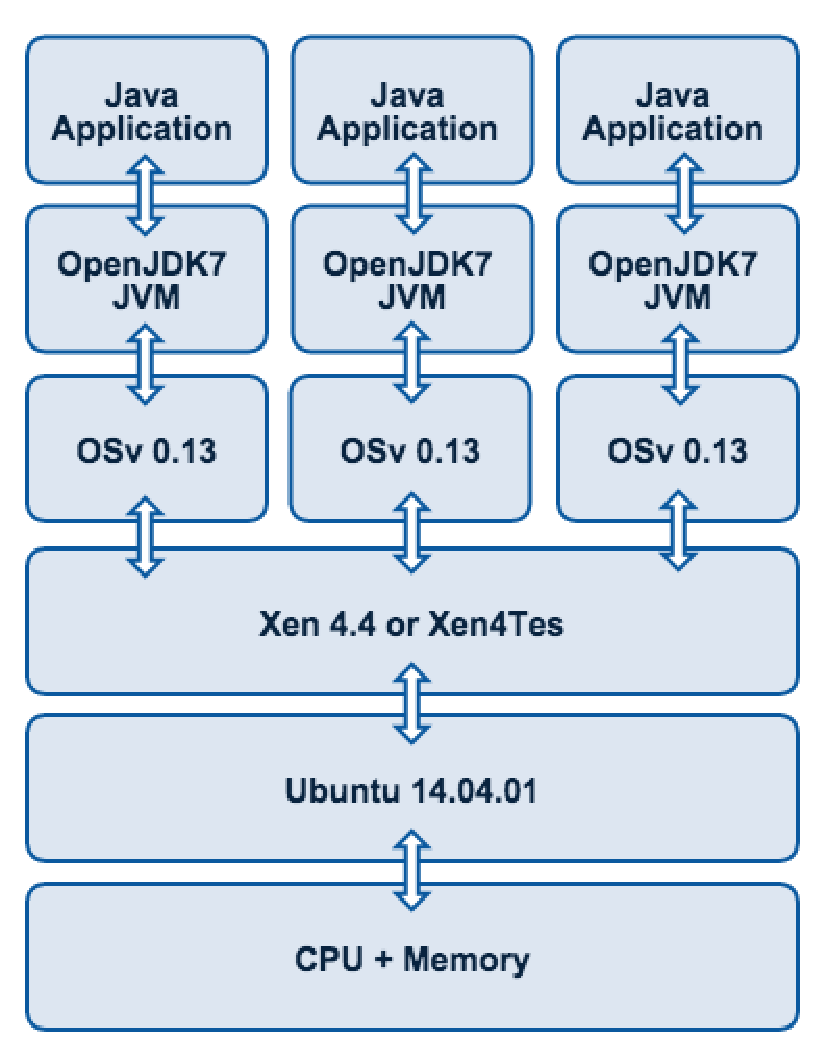
\epsfig{file=figures/dacaposetupdiagramcrop.eps, height=3.75in, width=3in}
\caption{The application layering of our experimental setup.}
\label{fig:dacaposetup}
\end{figure}

Figure~\ref{fig:dacaposetup} showcases our experimental setup. Our setup uses the OpenJDK7 implementation of the Java platform. We deploy our JVMs in Virtual Machines running the OS$^{v}$ 0.13 Operating System \cite{aviOSv2014}. OS$^{v}$ VMs are run as guest domains on the Xen 4.4 hypervisor \cite{barham2003xen}. A custom Xen hypervisor (Xen4Tess) featuring a prototype implementation of a gang-scheduled CPU Pool is also used for our gang-scheduling experiments. The hypervisor runs on a 2-socket machine with 2 Intel Core i7-920 processors at 2.67GHz (4 cores per socket, Hyperthreading off,  8 total CPUs). Our test machine has 12GB of physical memory and runs Ubuntu 14.04.01. Each Xen guest domain runs with 6 vCPUs serviced by 6-CPU pool and is allocated 512MB of memory. We reserve 2 CPUs and 3GB of memory for Domain-0.  

We only run a subset of the Dacapo benchmark suite in our experiments (avrora, jython, luindex, lusearch, xalan). This subset was chosen because other benchmarks within the suite have bugs when running within OS$^{v}$.

We run two separate experiments using Dacapo. First, we measure the overall performance difference between running JVM's in parallel with and without gang scheduling of CPU resources. In our second experiment, we wish to explore the performance of the JIT compiler's code profiler and optimizer in the warmup phase during parallel JVM load.

%TODO May need to change numbers in the following 2 paragraphs

\subsubsection{Experiment 1: Overall Performance}
For each benchmark in our subset, we run 1, 2, 4, 8, and 16 JVMs in parallel with maximum heapsizes 1x, 2x, 4x, and 8x times the minimum heapsize for the benchmark. The minimum heapsize for each benchmark is empirically determined by reducing the heapsize until an out of memory error occurs. We warmup our JVMs by running the benchmark for some number of iterations. The number of warmup iterations is empirically determined by calculating the average number of iterations needed until performance stabilizes. The execution times of the next 5 iterations after warmup are recorded and an arithmetic mean is reported as the benchmark runtime for each JVM. 
%TODO What we did for GS?

%TODO we may have changed this experiment

\subsubsection{Experiment 2: JIT Compiler Performance}
First, we run a single JVM in isolation with maximum heapsizes 1x, 2x, 4x, and 8x times the minimum heapsize for the benchmark. Similarly to Experiment 1, we record the execution times of the next 5 iterations after warmup and compute an arithmetic mean. Next we warm up a single JVM with the same heapsizes under the load of 15 other JVMs running in parallel. After warmup, we kill the other JVMs and run the single JVM in isolation; again computing the arithmetic mean of the execution times of the next 5 iterations. We repeat these steps for each combination of benchmark and heapsize 5 times recording 5 data points per combination.
%TODO What we did for GS?

\subsection{Results}

%Because tables cannot be split across pages, the best
%placement for them is typically the top of the page
%nearest their initial cite.  To
%ensure this proper ``floating'' placement of tables, use the
%environment \textbf{table} to enclose the table's contents and
%the table caption.  The contents of the table itself must go
%in the \textbf{tabular} environment, to
%be aligned properly in rows and columns, with the desired
%horizontal and vertical rules.  Again, detailed instructions
%on \textbf{tabular} material
%is found in the \textit{\LaTeX\ User's Guide}.
%
%Immediately following this sentence is the point at which
%Table 1 is included in the input file; compare the
%placement of the table here with the table in the printed
%dvi output of this document.
%
\begin{table}
\centering
\caption{Standard Deviations of Dacapo Benchmarks}
\begin{tabular}{|c|c|l|} \hline
Benchmark&Standard Deviation&Variance\\ \hline
avrora &1000&100\\
\hline\end{tabular}
\end{table}

%To set a wider table, which takes up the whole width of
%the page's live area, use the environment
%\textbf{table*} to enclose the table's contents and
%the table caption.  As with a single-column table, this wide
%table will ``float" to a location deemed more desirable.
%Immediately following this sentence is the point at which
%Table 2 is included in the input file; again, it is
%instructive to compare the placement of the
%table here with the table in the printed dvi
%output of this document.

%\begin{table*}
%\centering
%\caption{Some Typical Commands}
%\begin{tabular}{|c|c|l|} \hline
%Command&A Number&Comments\\ \hline
%\texttt{{\char'134}alignauthor} & 100& Author alignment\\ \hline
%\texttt{{\char'134}numberofauthors}& 200& Author enumeration\\ \hline
%\texttt{{\char'134}table}& 300 & For tables\\ \hline
%\texttt{{\char'134}table*}& 400& For wider tables\\ \hline\end{tabular}
%\end{table*}
%% end the environment with {table*}, NOTE not {table}!

\section{YCSB}

%TODO Things we might want to talk about: communication, synchronization, interactivity/responsiveness/timing/QoS requirements

\subsection{Experimental Setup}

\subsection{Results}
%Like tables, figures cannot be split across pages; the
%best placement for them
%is typically the top or the bottom of the page nearest
%their initial cite.  To ensure this proper ``floating'' placement
%of figures, use the environment
%\textbf{figure} to enclose the figure and its caption.
%
%This sample document contains examples of \textbf{.eps}
%and \textbf{.ps} files to be displayable with \LaTeX.  More
%details on each of these is found in the \textit{Author's Guide}.

\begin{figure}
\centering
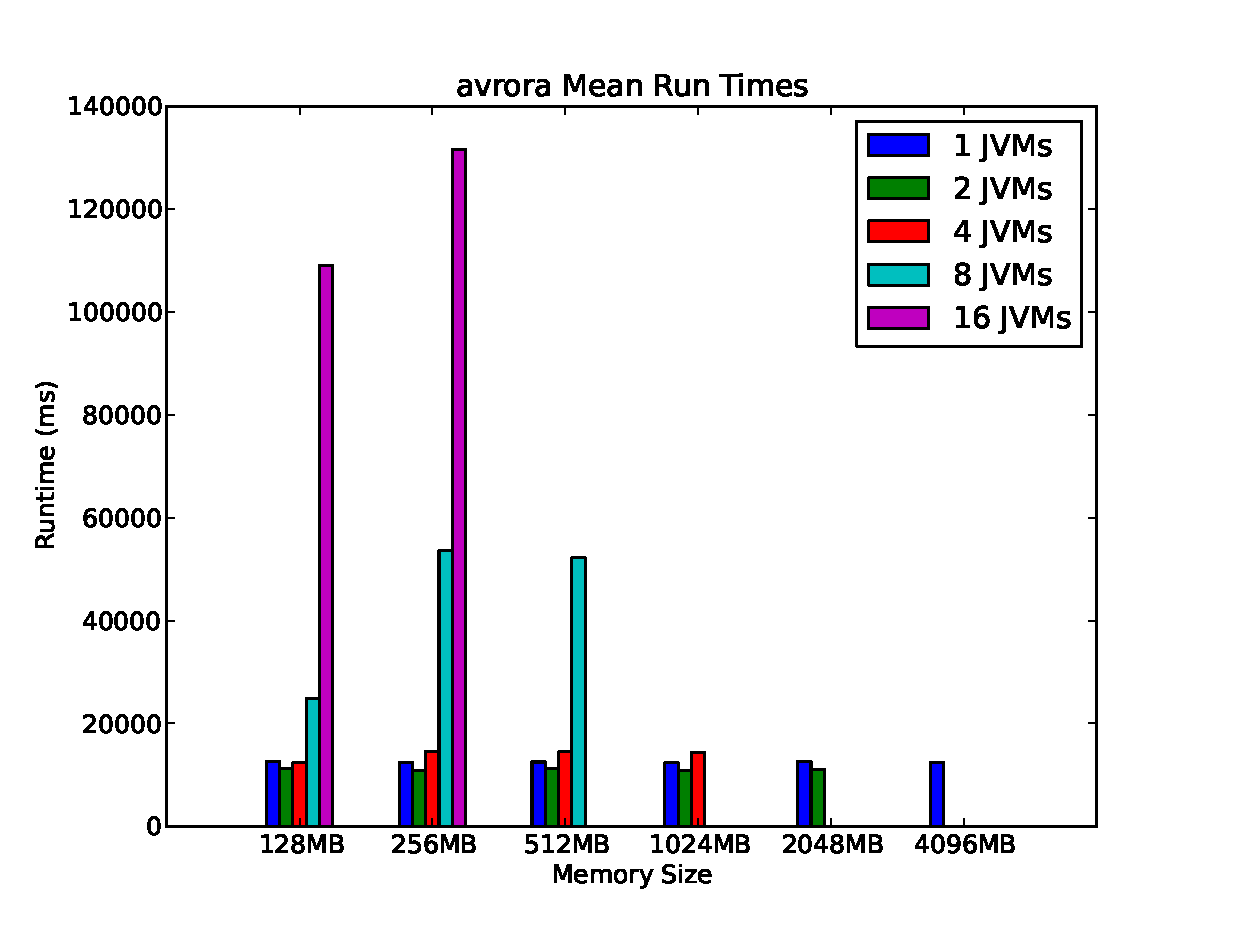
\epsfig{file=figures/avrora.eps, height=2in, width=3in}
\caption{A sample graphic (.eps format)
that has been resized with the \texttt{epsfig} command.}
\end{figure}

%As was the case with tables, you may want a figure
%that spans two columns.  To do this, and still to
%ensure proper ``floating'' placement of tables, use the environment
%\textbf{figure*} to enclose the figure and its caption.
%and don't forget to end the environment with
%{figure*}, not {figure}!

\begin{figure*}
\centering
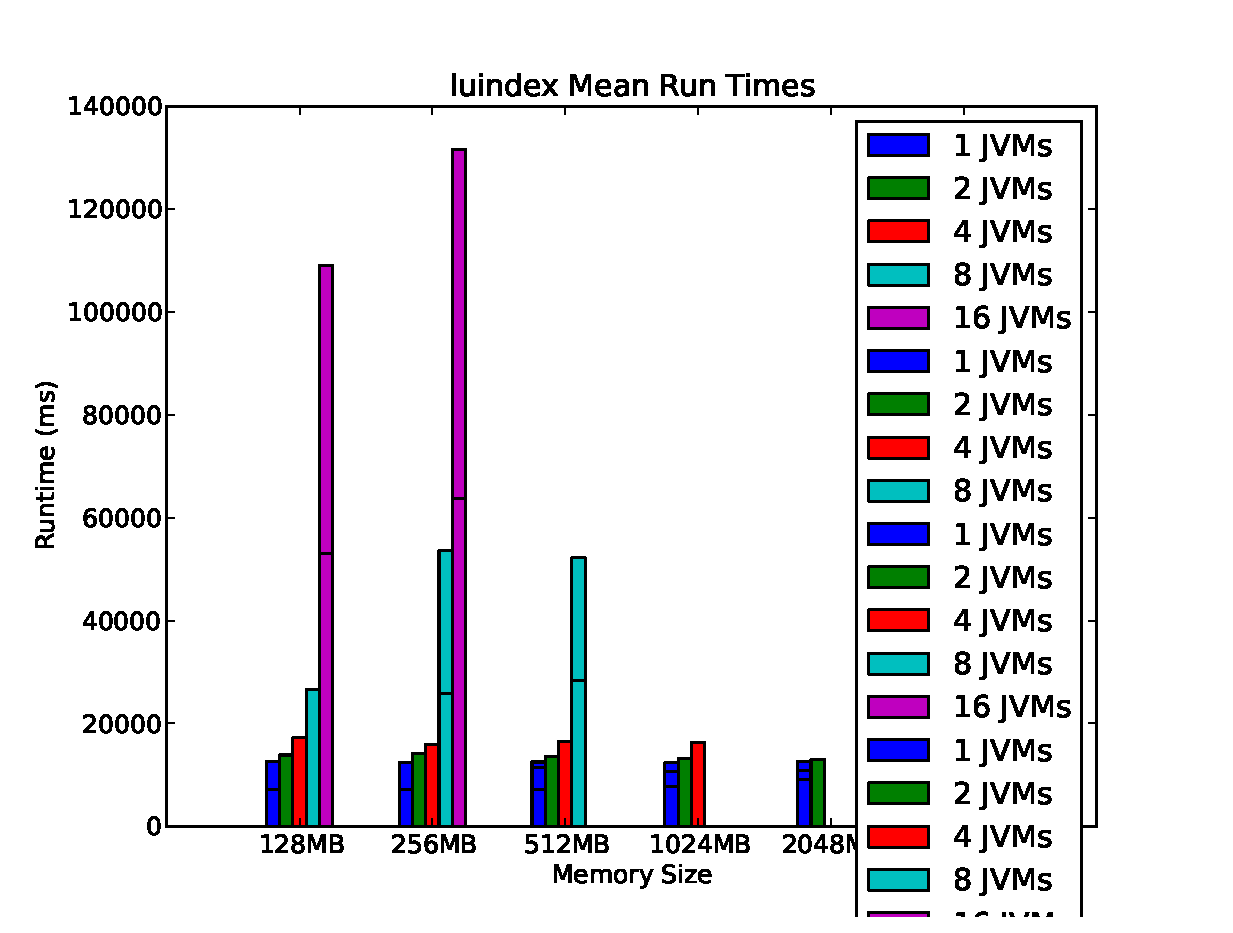
\epsfig{file=figures/luindex.eps}
\caption{A sample black and white graphic (.eps format)
that needs to span two columns of text.}
\end{figure*}

\section{Future Work}

Figure out what kind of workload it would take in order for interference to become a problem.

\section{Related Work}

%TODO Either defend against "Gang scheduling isn't worth it yet" paper or (possibly?) use it as an explanation.

\section{Conclusion}

%TODO Things we might want to talk about: communication, synchronization, interactivity/responsiveness/timing/QoS requirements

%ACKNOWLEDGMENTS are optional
\section{Acknowledgments}
Martin
Nathan
Eric

% The following two commands are all you need in the
% initial runs of your .tex file to
% produce the bibliography for the citations in your paper.
\bibliographystyle{abbrv}
\bibliography{JVMTesselation}  % sigproc.bib is the name of the Bibliography in this case
% You must have a proper ".bib" file
%  and remember to run:
% latex bibtex latex latex
% to resolve all references
%
% ACM needs 'a single self-contained file'!
%

\balancecolumns
\end{document}
